\section{Simulation and Results analysis}

In this section are presented the simulations performed on the LNA circuit in the three technologies mentioned before, including the analysis of the gain, noise figure, and input/output impedance. The simulations were conducted using LTSpice and Cadence, and the results are compared with theoretical expectations, and the technologies are compared in terms of performance metrics.

\subsection{Simulation for 350 nm Technology}

The simulations for this technology were done in LTSpice.
\subsubsection{1:1 $g_m$ ratio}

The results of the s parameters for the 350 nm technology with a 1:1 $g_m$ ratio are shown in Figure \ref{fig:350nm_1to1}. 
\begin{figure}[H]
    \centering
    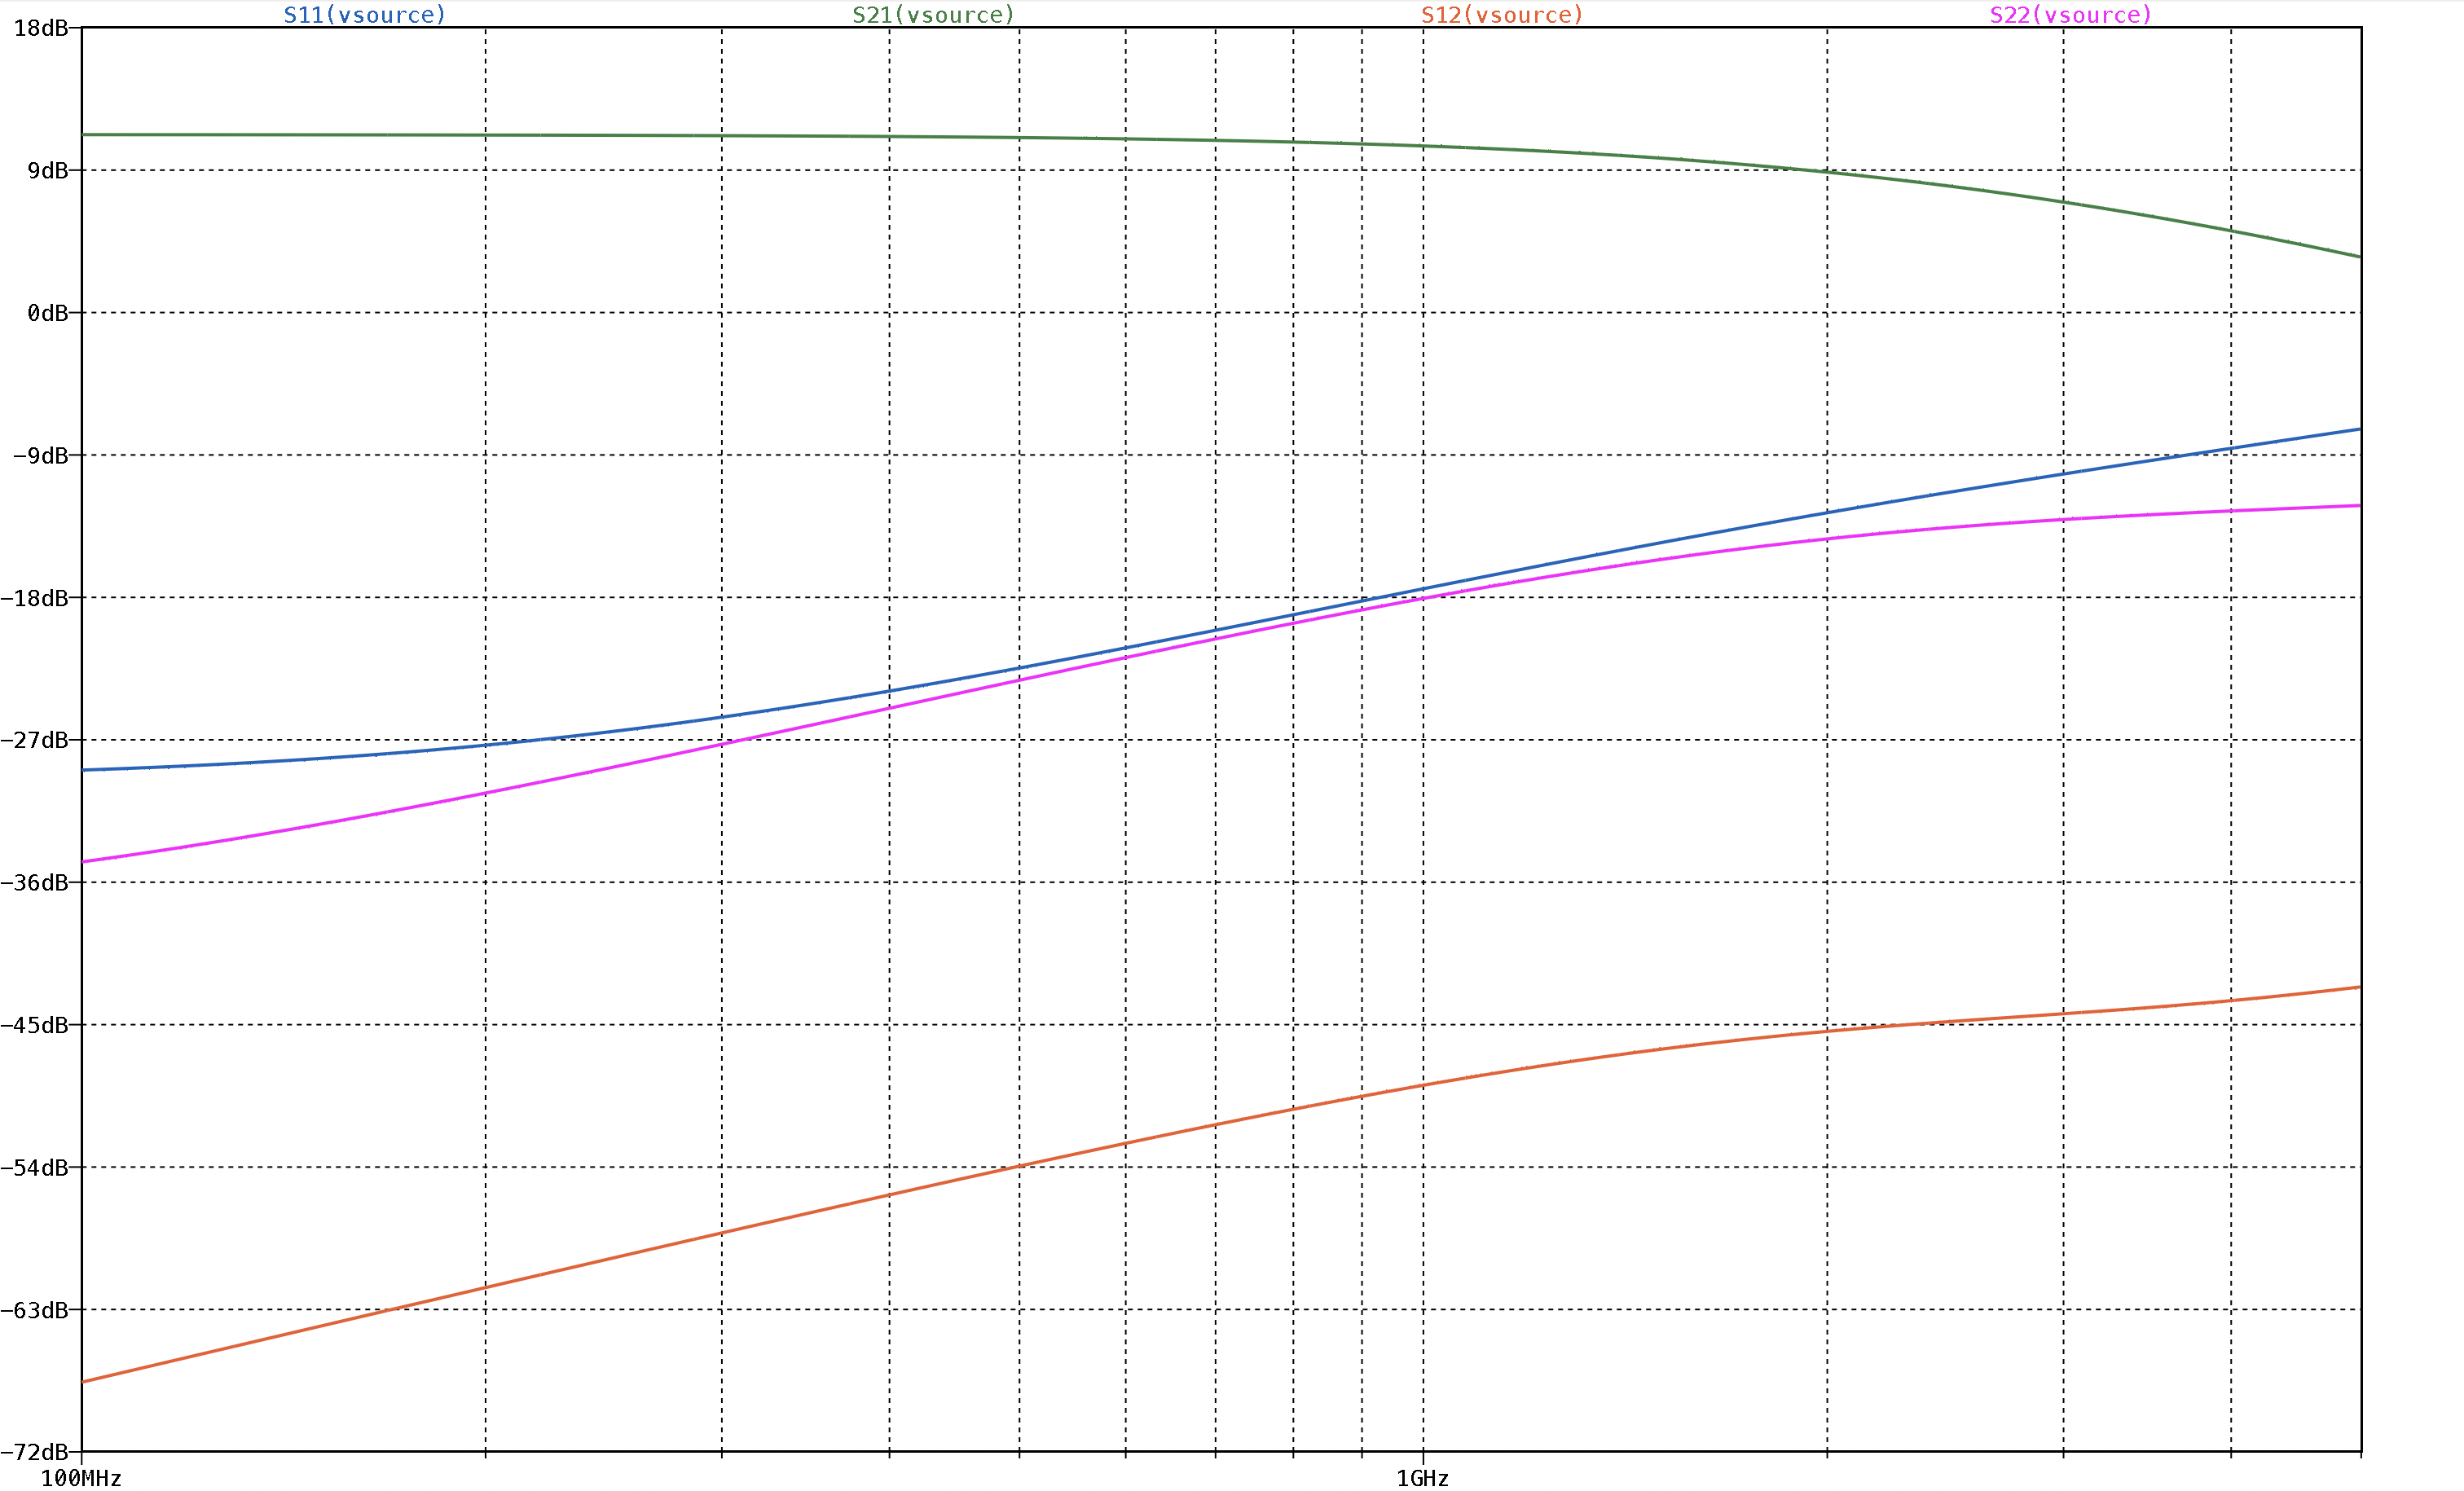
\includegraphics[width=0.8\textwidth]{Images/3501to1SParam.png}
    \caption{S parameters simulation for 350 nm Technology with 1:1 $g_m$ Ratio}
    \label{fig:350nm_1to1}
\end{figure}

The results for the input and output impedances are shown in Figure \ref{fig:350nm_1to1-Z}.

\begin{figure}[H]
    \centering
    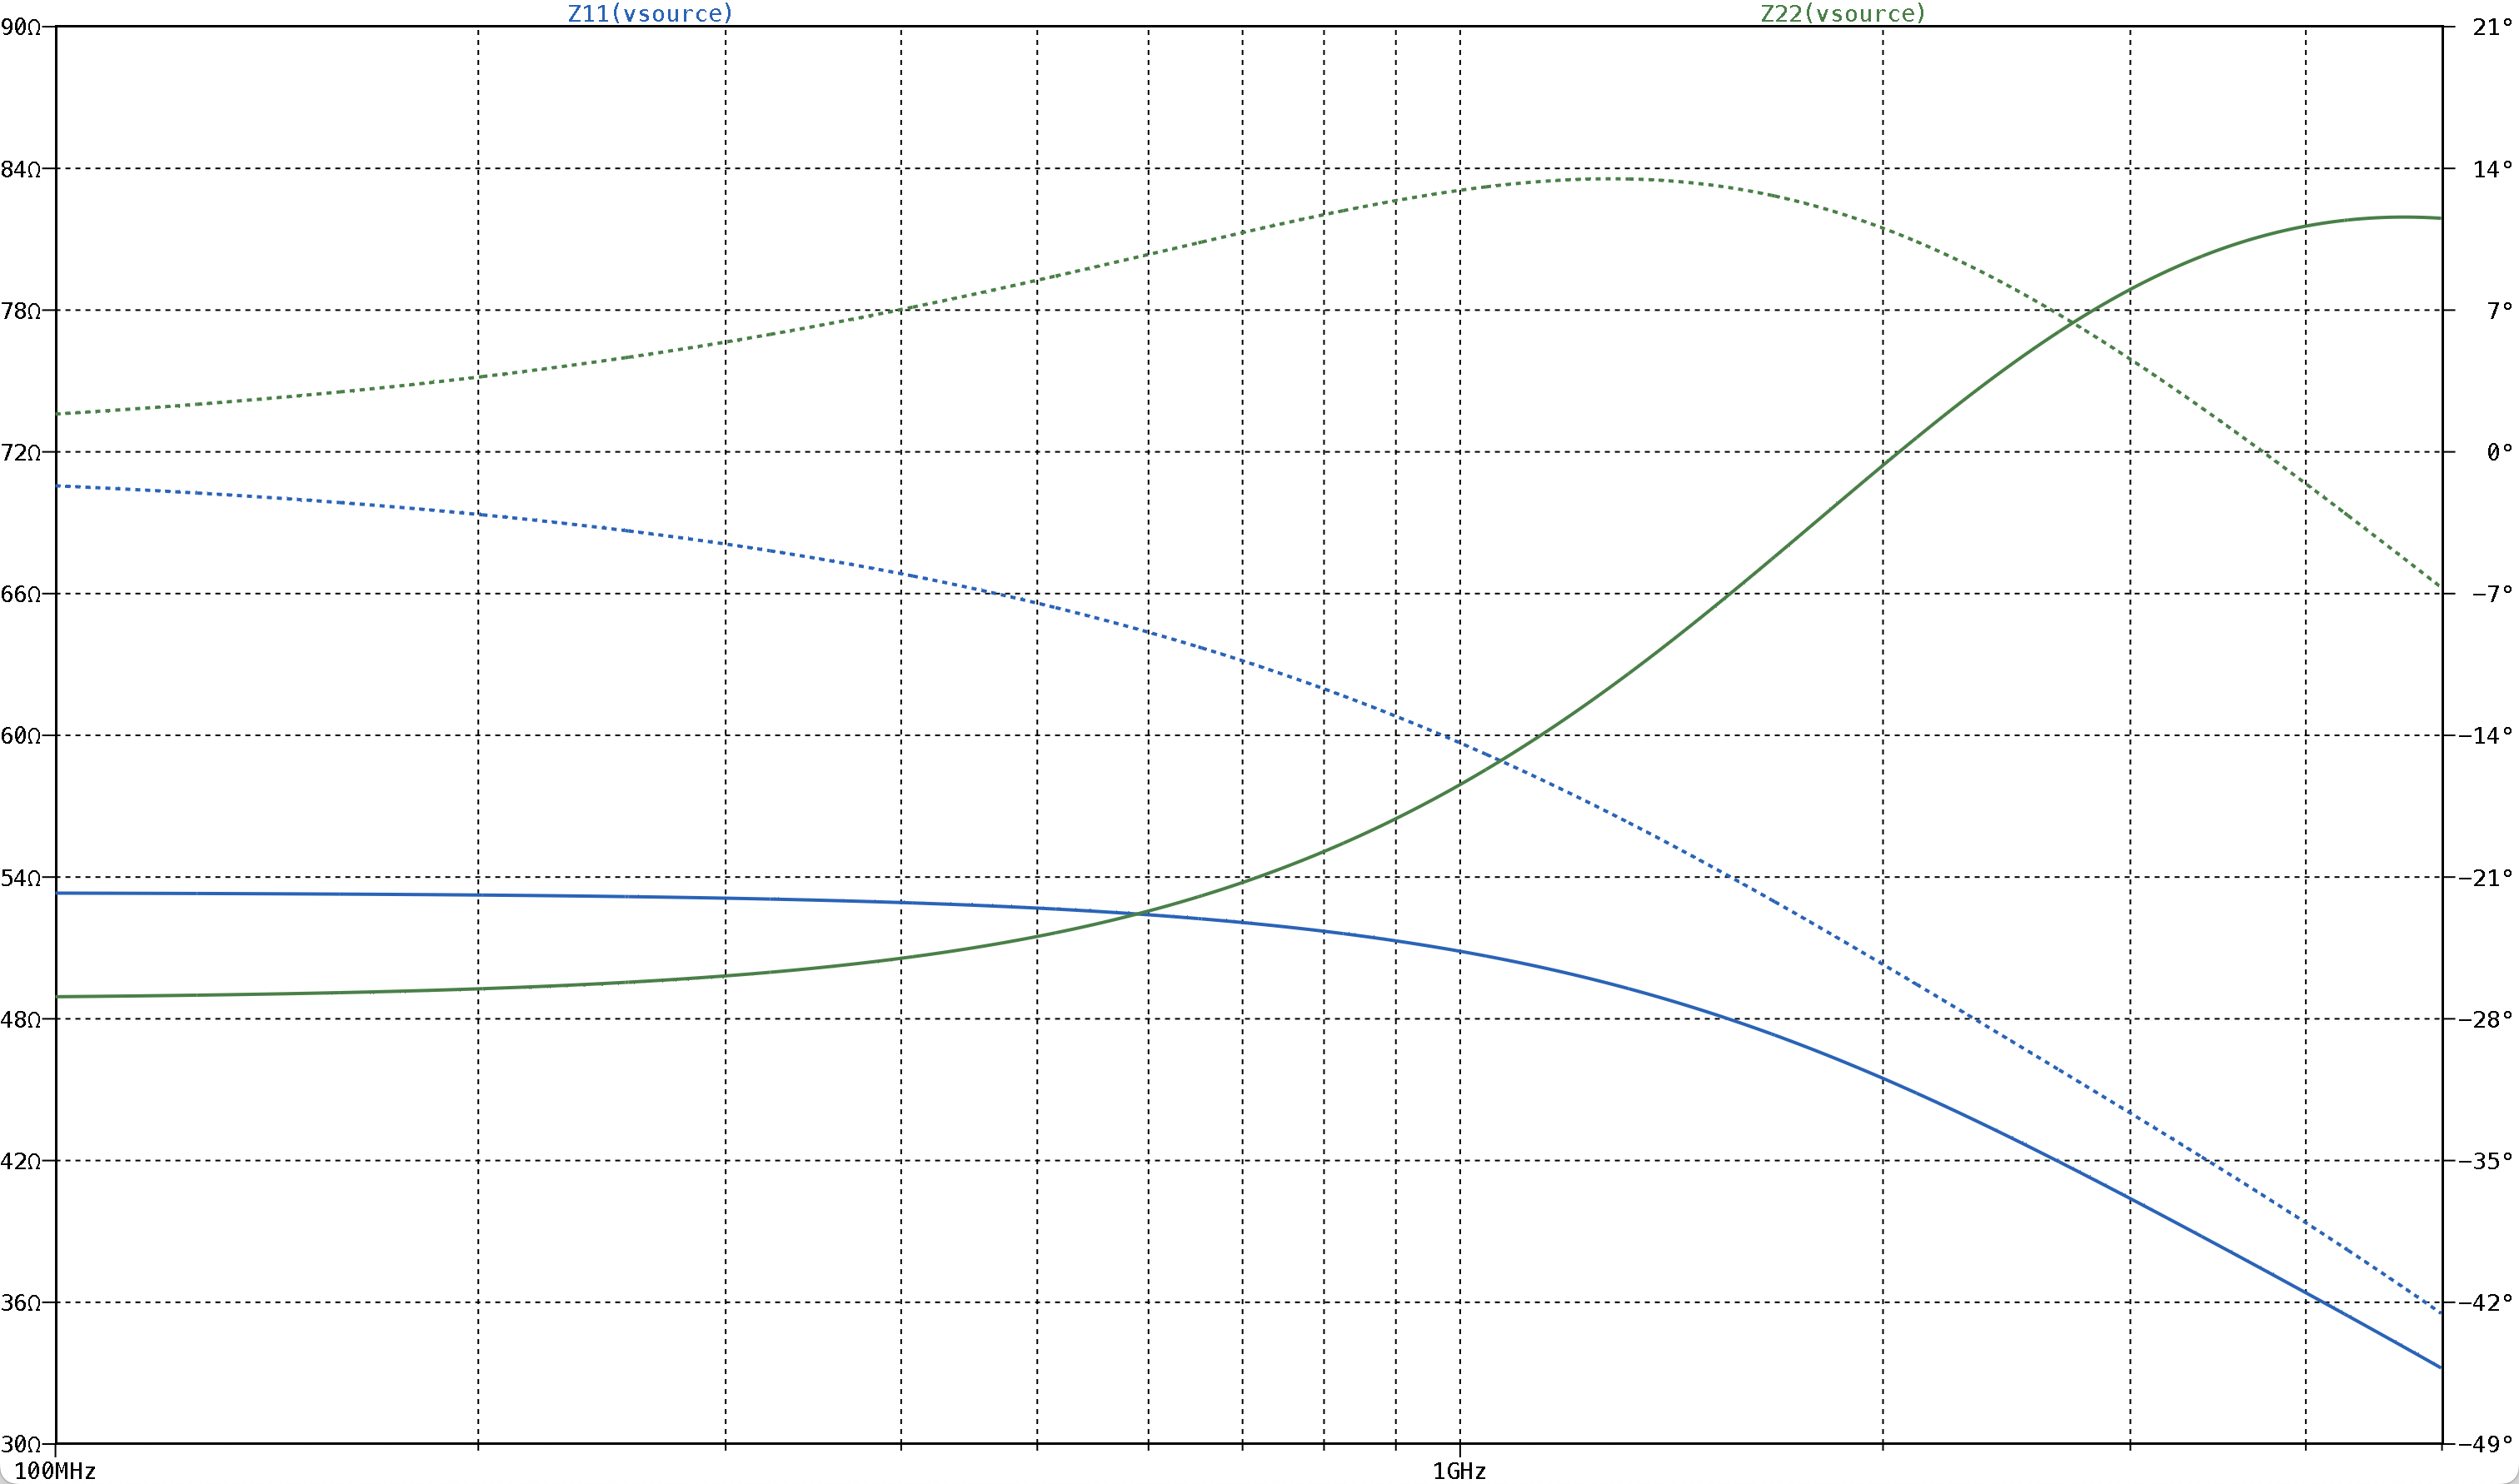
\includegraphics[width=0.8\textwidth]{Images/3501to1ZParam.png}
    \caption{Input and Output Impedances for 350 nm Technology with 1:1 $g_m$ Ratio}
    \label{fig:350nm_1to1-Z}
\end{figure}

Lastly the simulation of the noise factor is shown in Figure \ref{fig:350nm_1to1-NF}.
\begin{figure}[H]
    \centering
    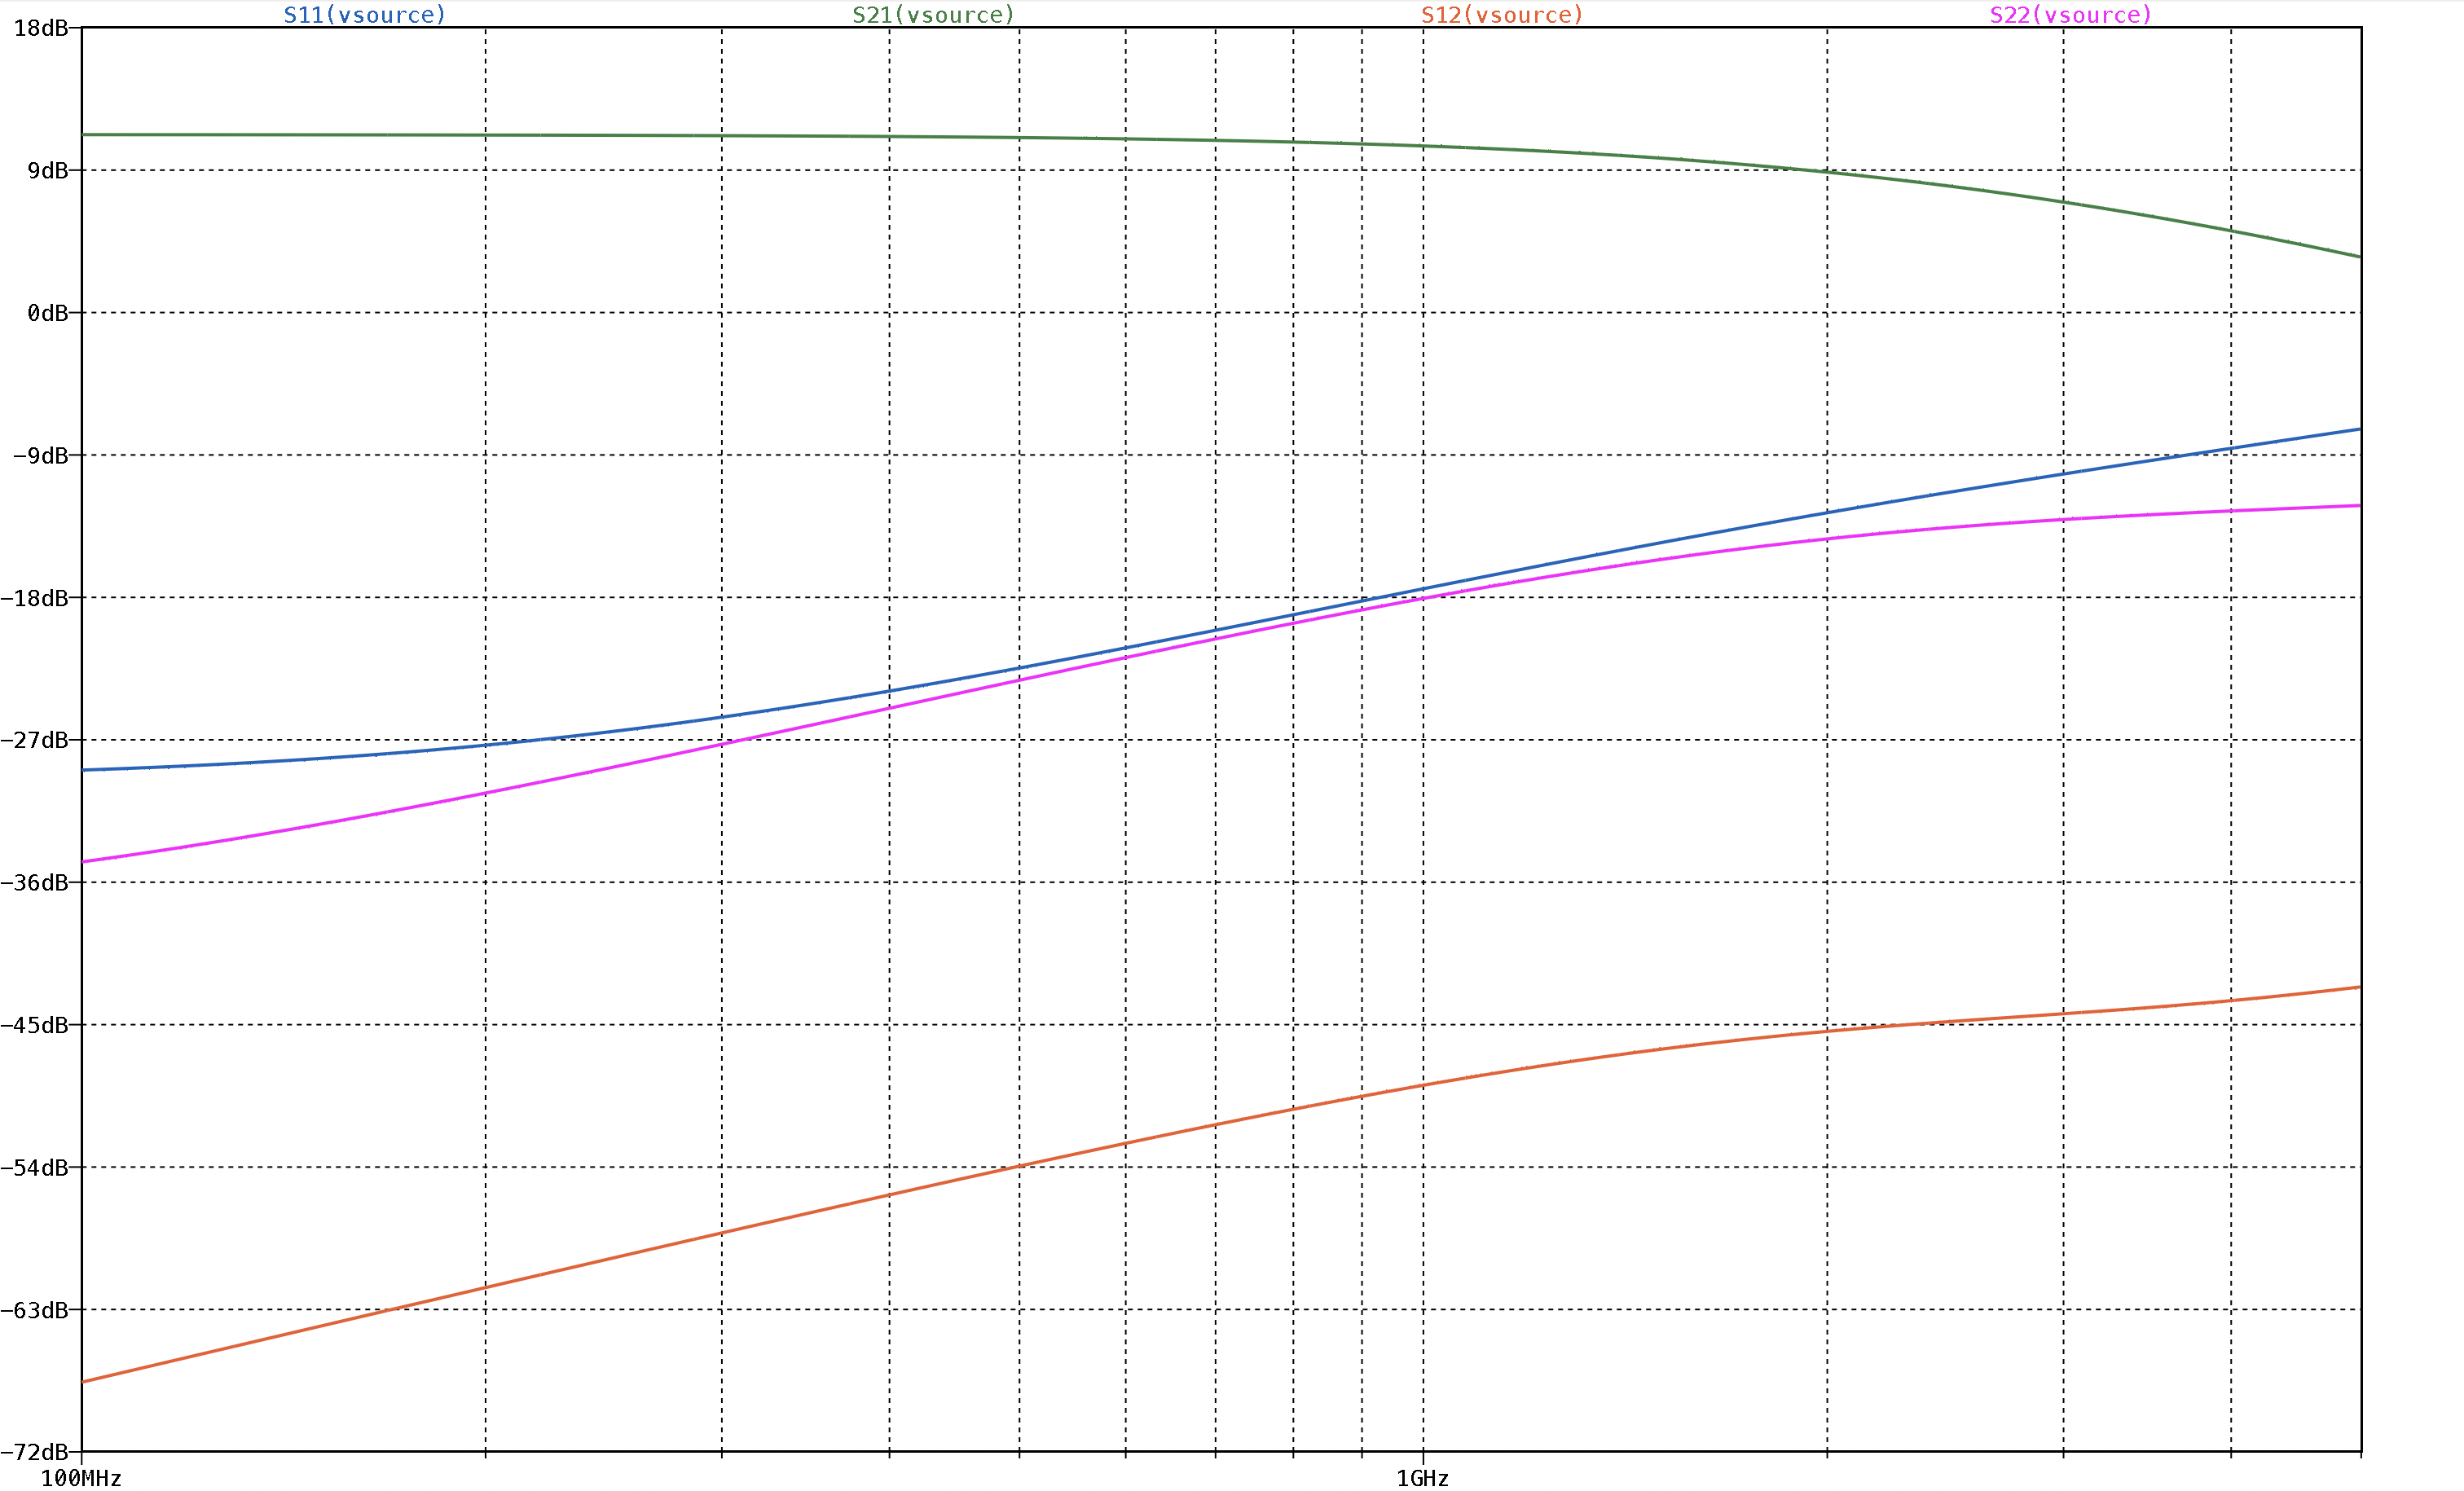
\includegraphics[width=0.8\textwidth]{Images/3501to1SParam.png}
    \caption{Noise Figure for 350 nm Technology with 1:1 $g_m$ Ratio}
    \label{fig:350nm_1to1-NF}
\end{figure}

\begin{table}[H]
    \centering
    \caption{Simulation Results for 350 nm Technology with 1:1 $g_m$ Ratio}
    \begin{tabularx}{\textwidth}{>{\centering\arraybackslash}X >{\centering\arraybackslash}X }
        \toprule
        \textbf{Parameter} & \textbf{Value}\\
        \midrule
        Gain (S21) & \SI{10.52}{\decibel} \\
        \midrule
        Noise Figure (NF) & \SI{3.19}{\decibel} \\
        \midrule
        Input Impedance (Z11) & \SI{50.84}{\ohm} \\
        \midrule
        Output Impedance (Z22) & \SI{57.94}{\ohm} \\
        \bottomrule
    \end{tabularx}
    \label{tab:350nm_1to1_results}
\end{table}
\subsubsection{1:3 $g_m$ ratio}

The results of the s parameters for the 350 nm technology with a 1:3 $g_m$ ratio are shown in Figure \ref{fig:350nm_1ton}. 
\begin{figure}[H]
    \centering
    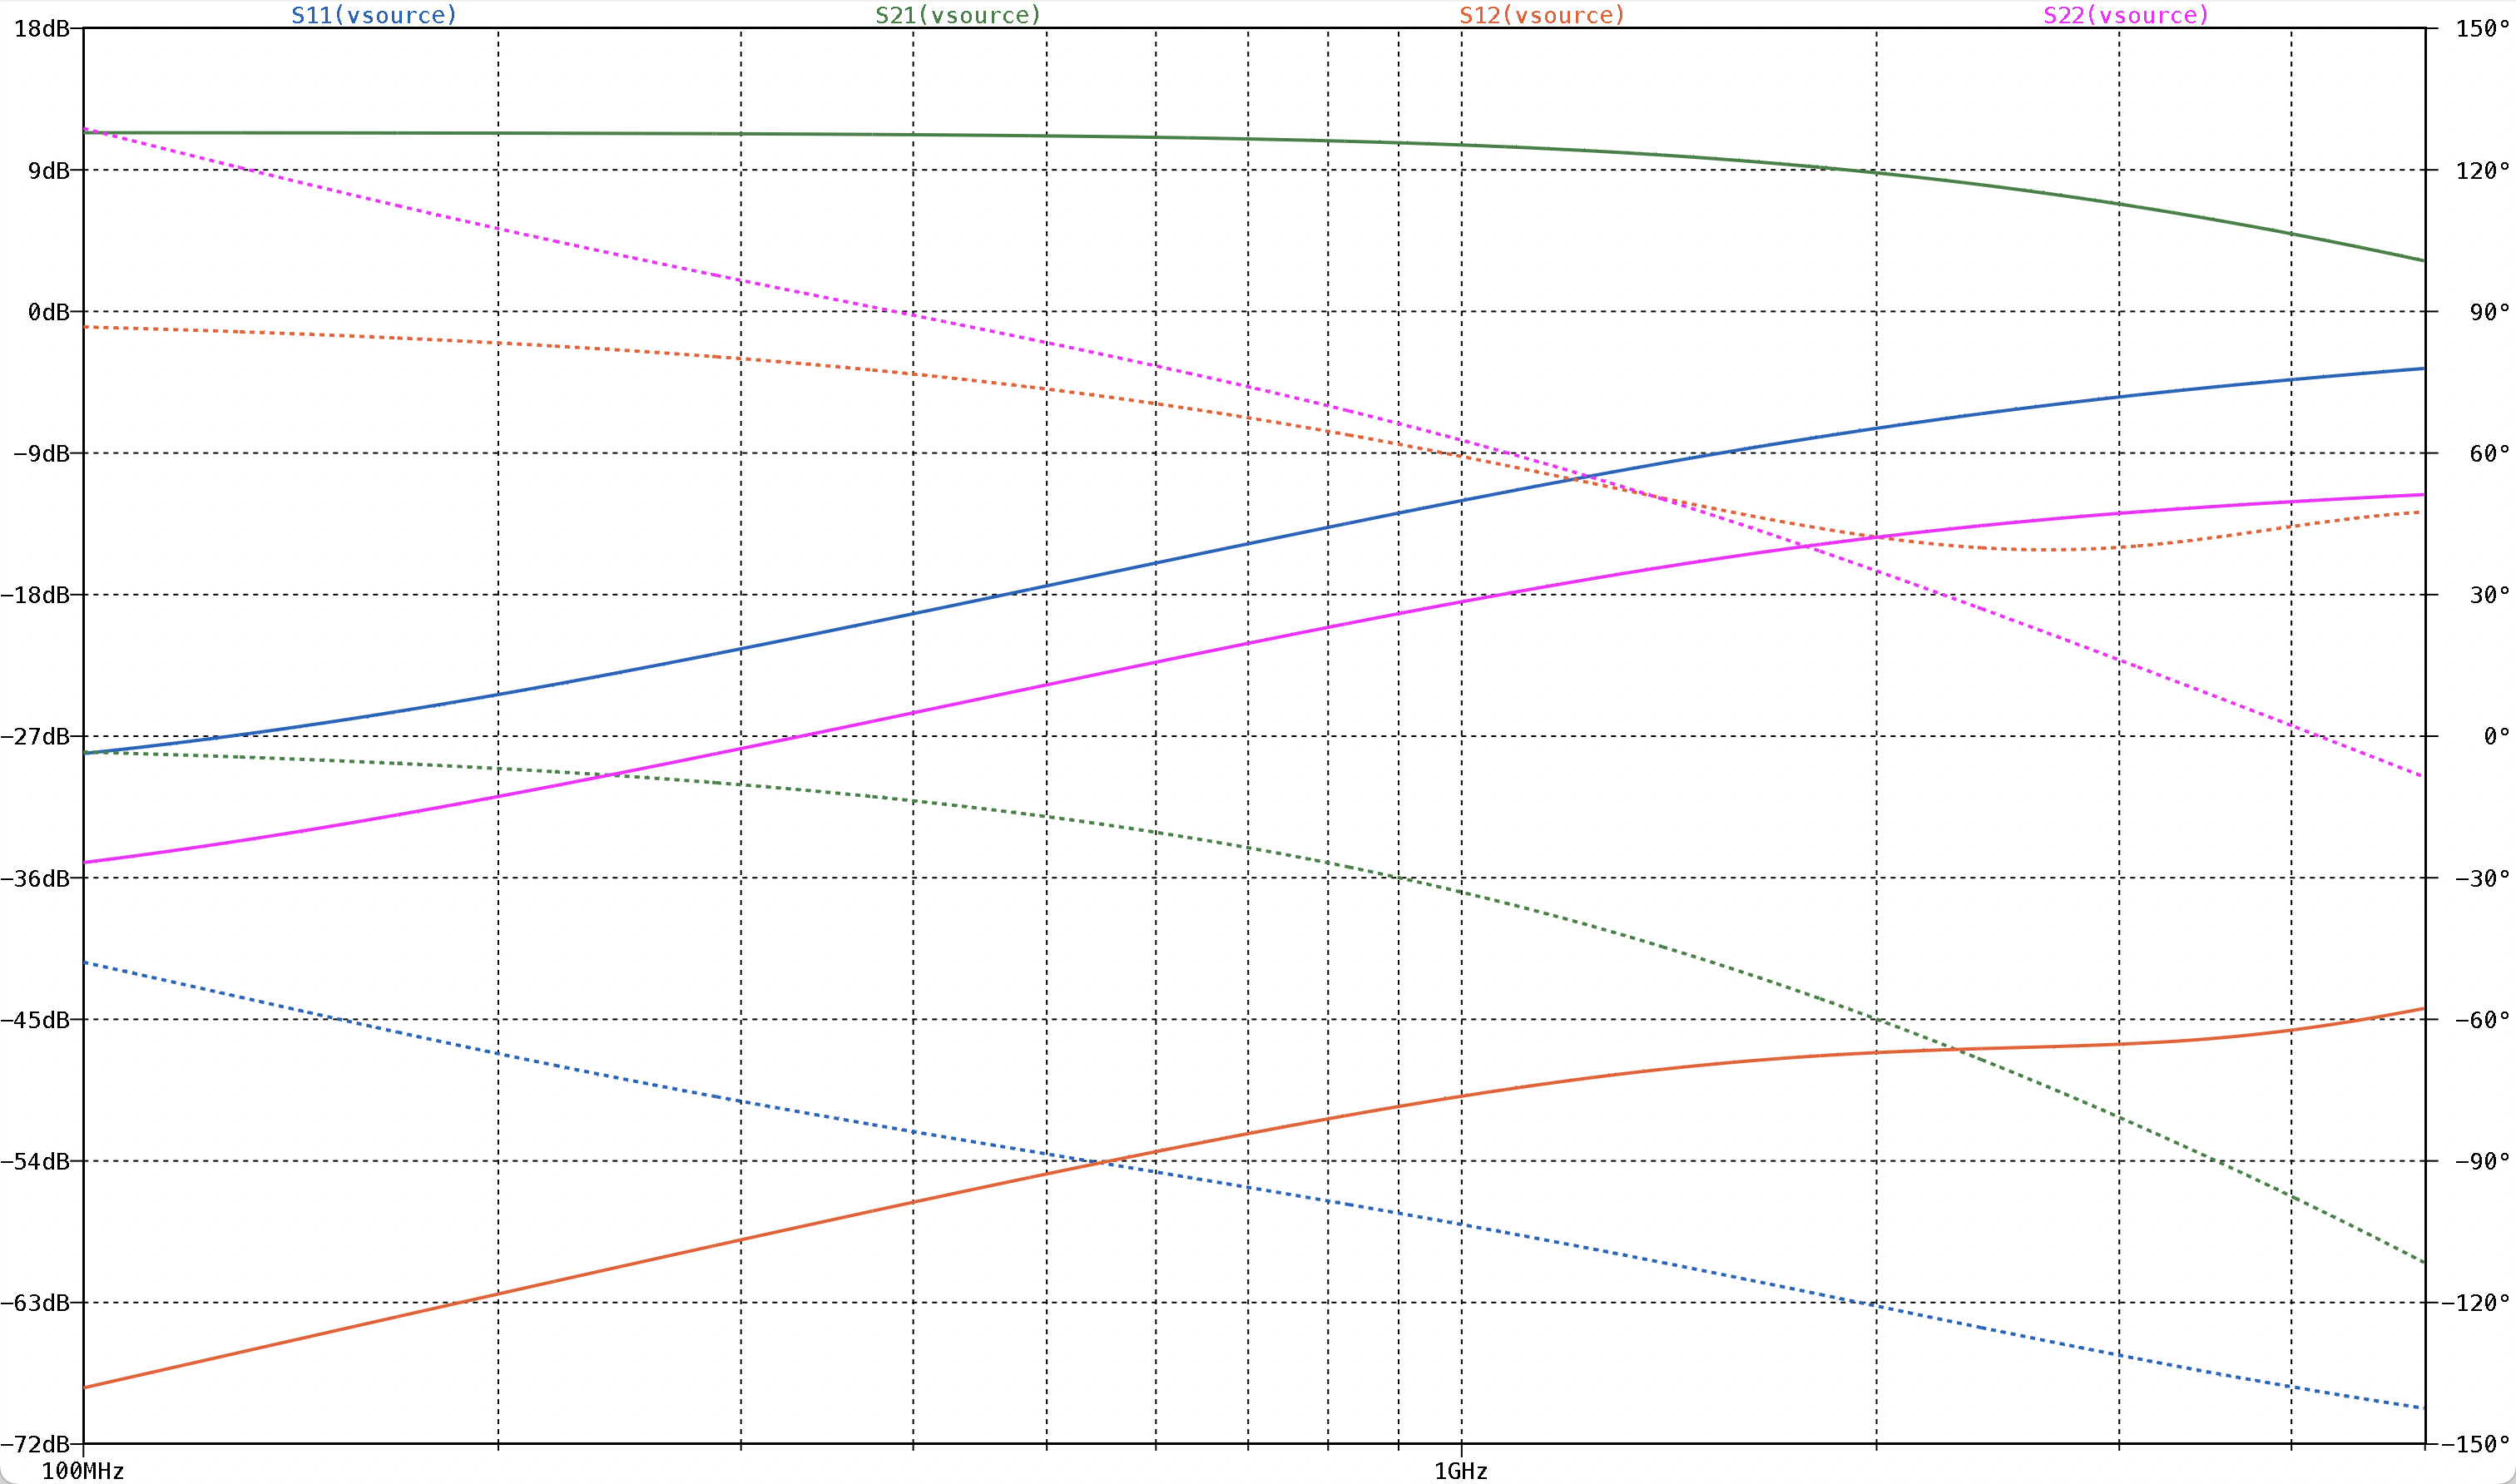
\includegraphics[width=0.8\textwidth]{Images/3501to3SParam.png}
    \caption{S parameters simulation for 350 nm Technology with 1:3 $g_m$ Ratio}
    \label{fig:350nm_1ton}
\end{figure}

The results for the input and output impedances are shown in Figure \ref{fig:350nm_1to1-Z}.

\begin{figure}[H]
    \centering
    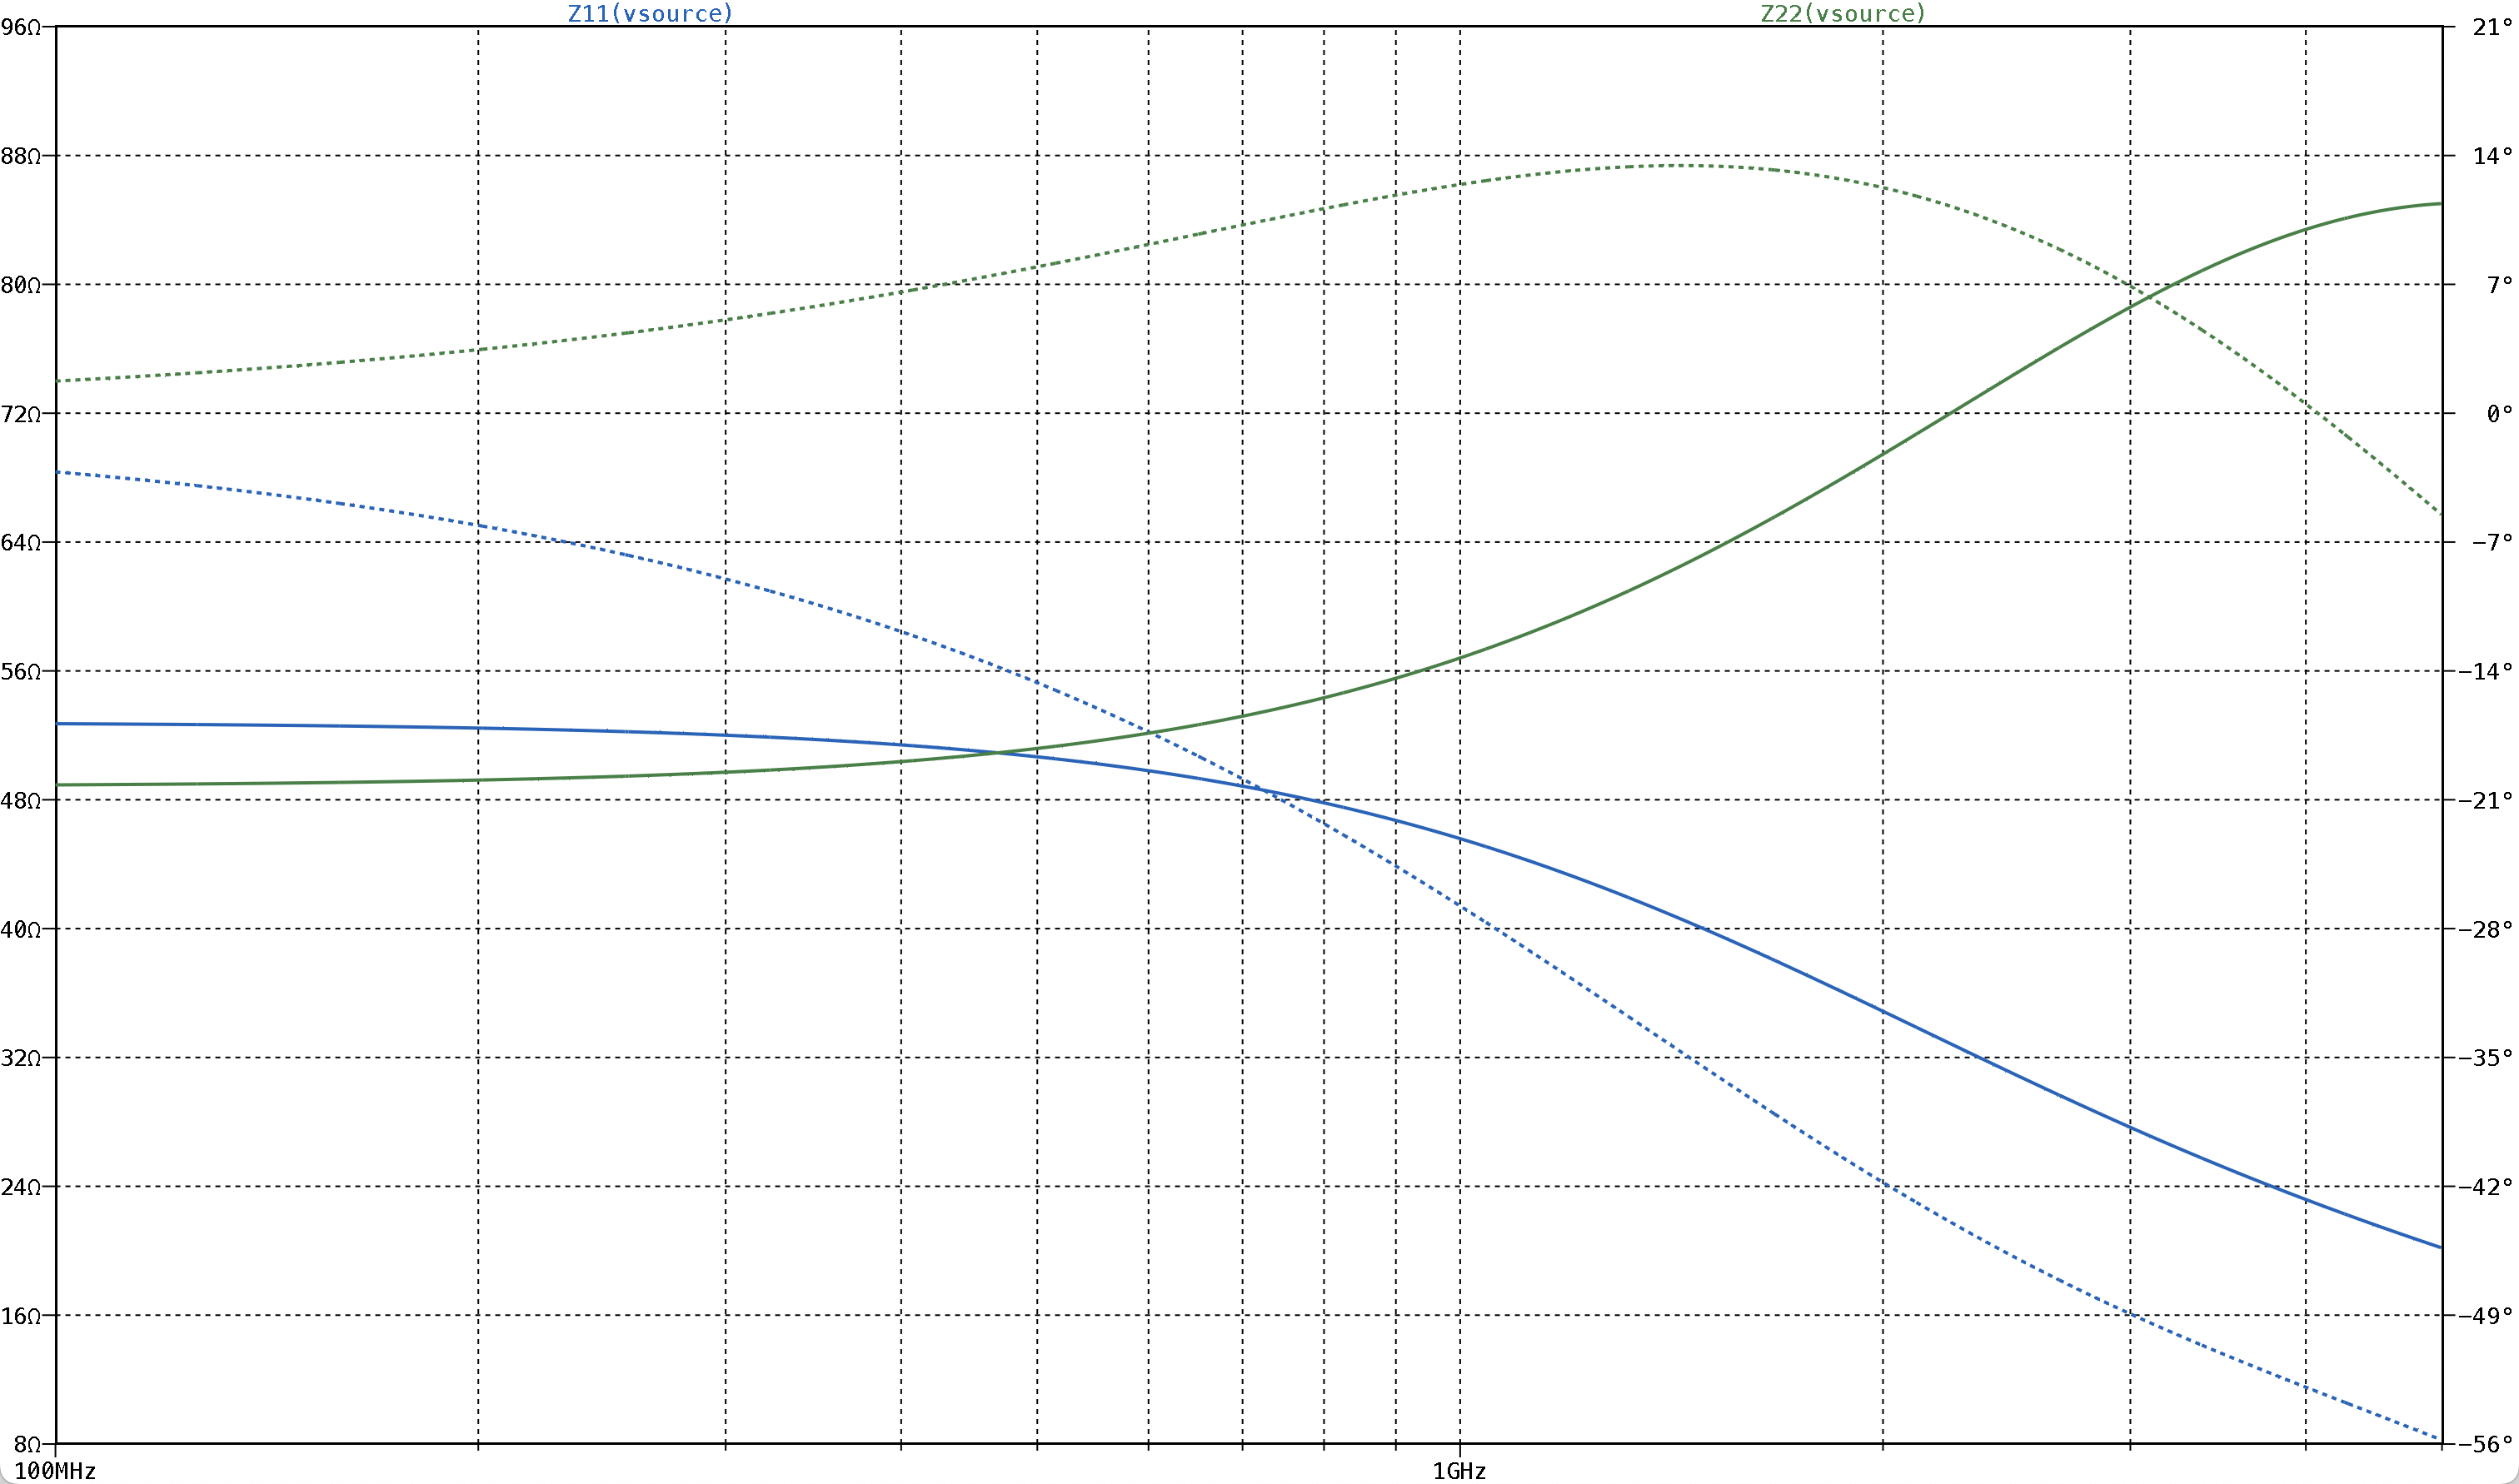
\includegraphics[width=0.8\textwidth]{Images/3501to3ZParam.png}
    \caption{Input and Output Impedances for 350 nm Technology with 1:3 $g_m$ Ratio}
    \label{fig:350nm_1ton-Z}
\end{figure}

Lastly the simulation of the noise factor is shown in Figure \ref{fig:350nm_1ton-NF}.
\begin{figure}[H]
    \centering
    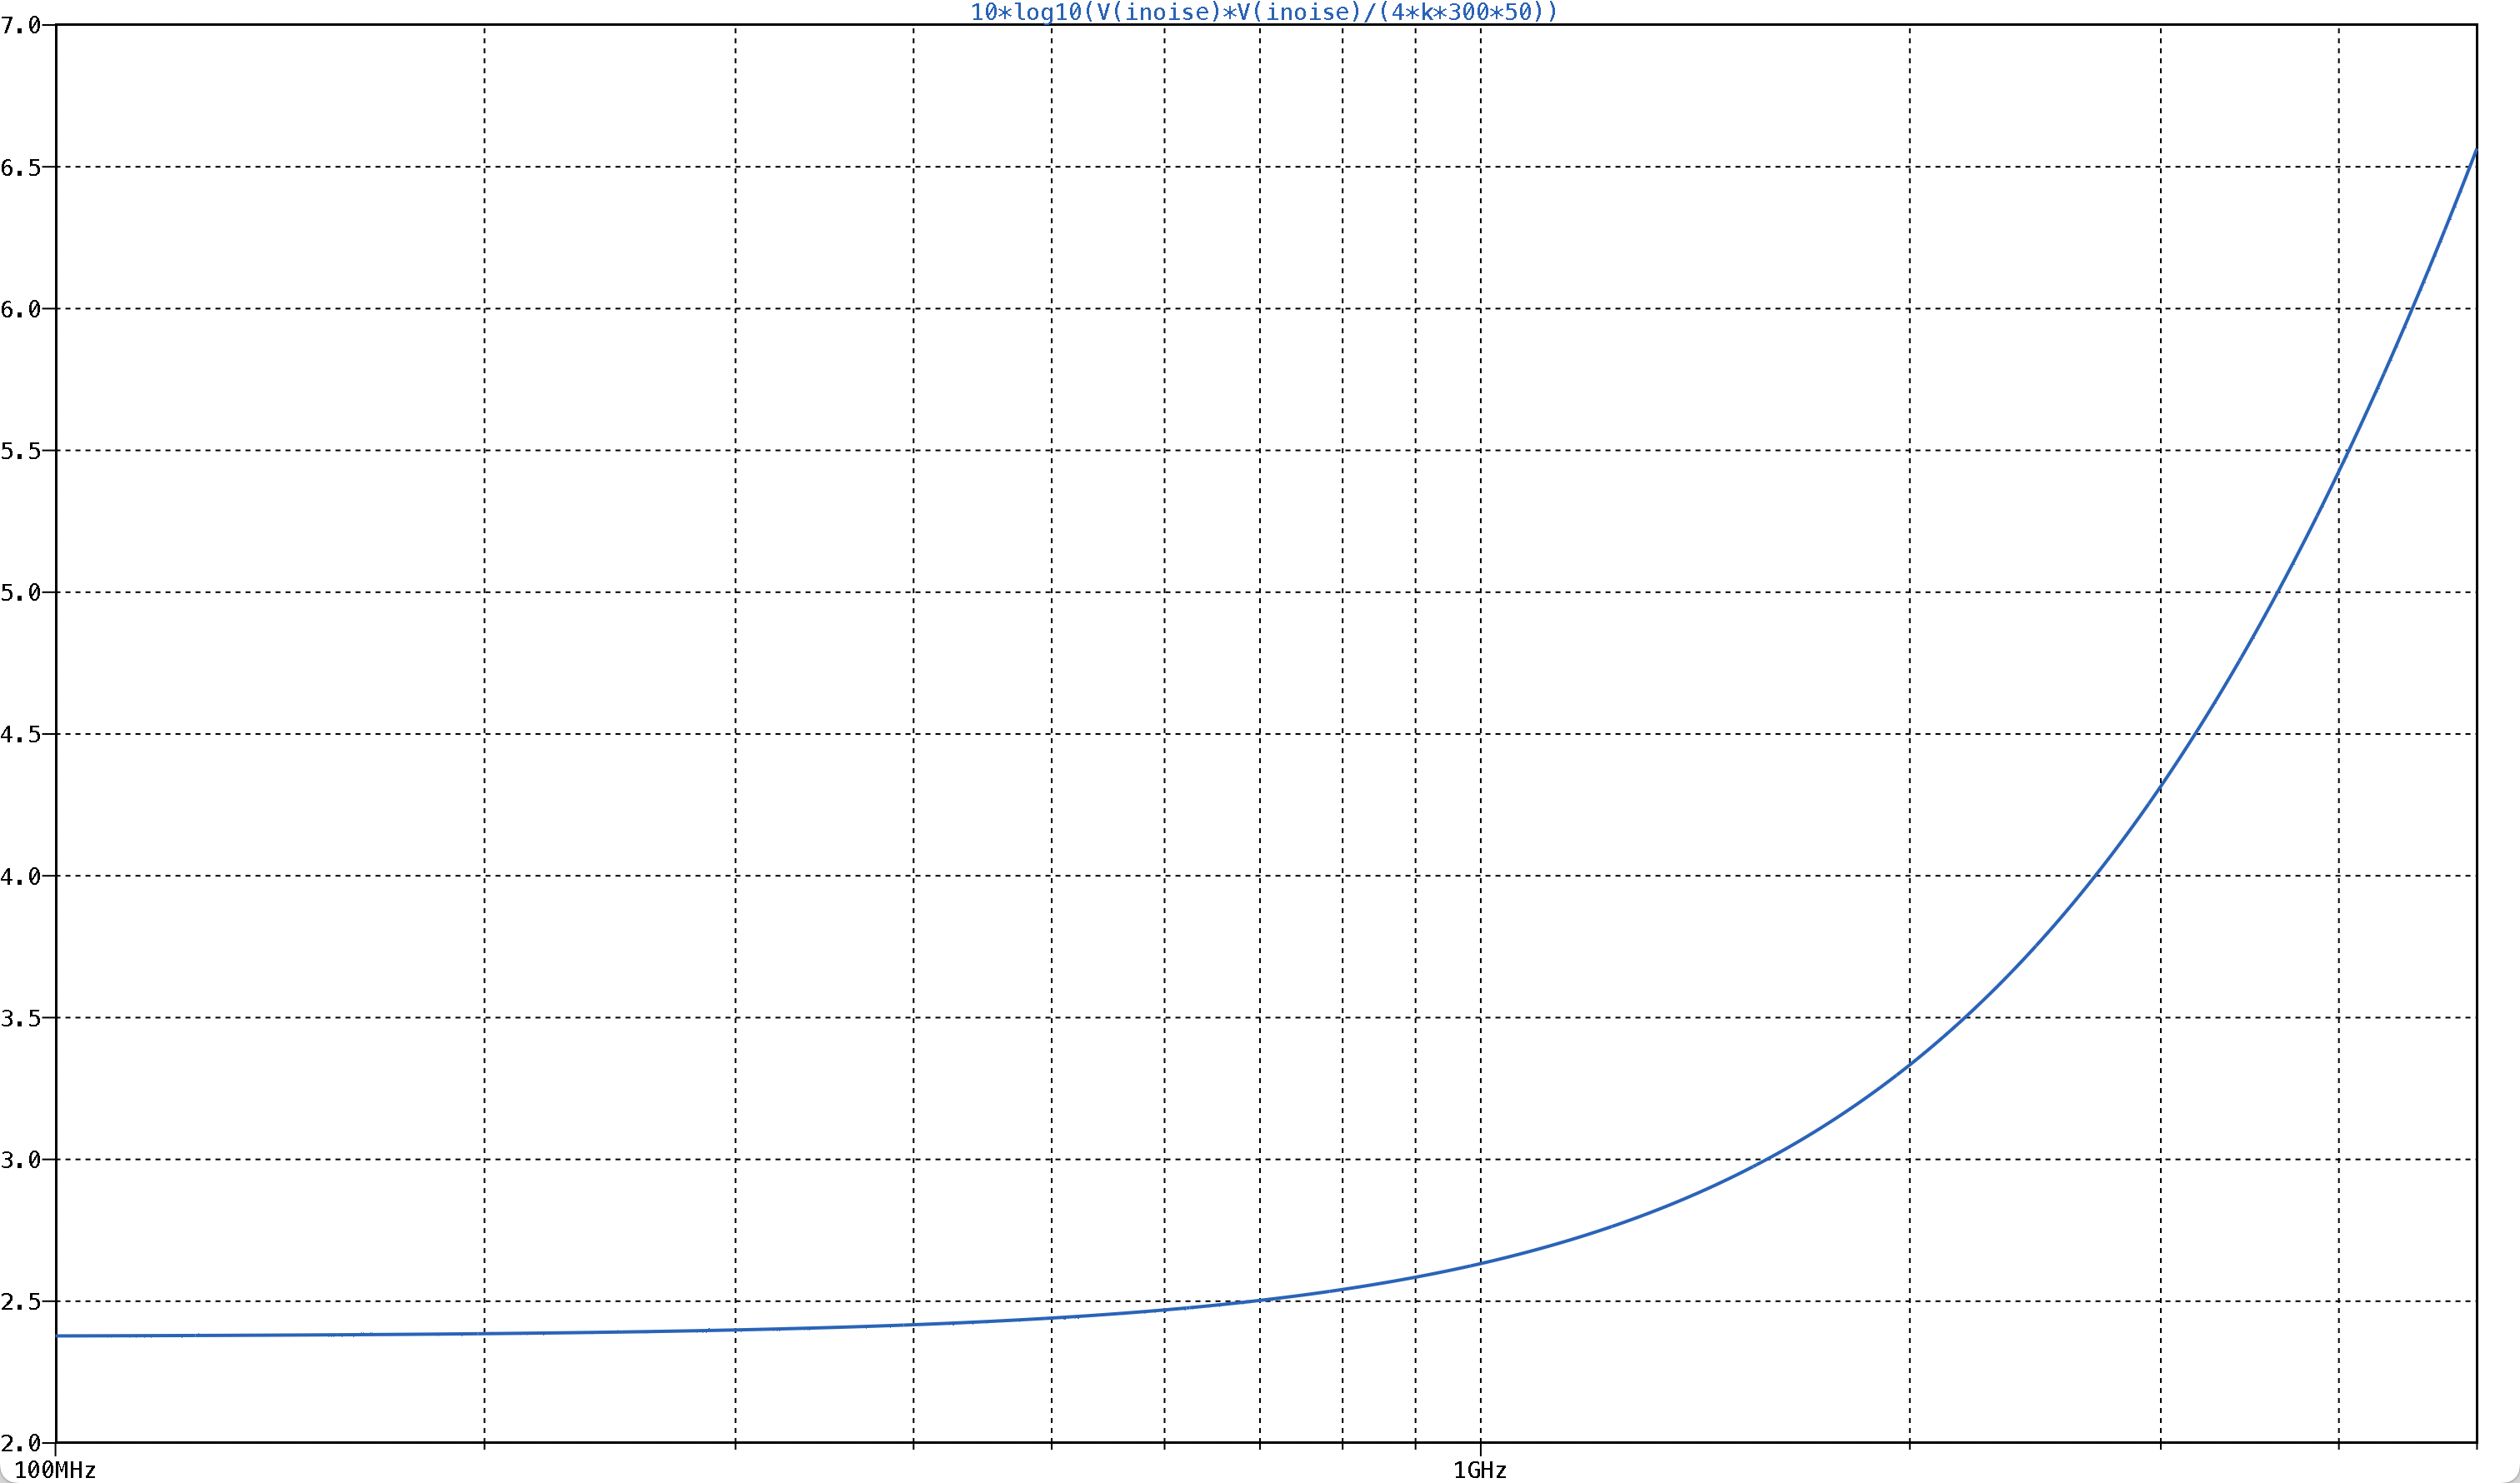
\includegraphics[width=0.8\textwidth]{Images/3501to3Noise.png}
    \caption{Noise Figure for 350 nm Technology with 1:3 $g_m$ Ratio}
    \label{fig:350nm_1ton-NF}
\end{figure}

\begin{table}[H]
    \centering
    \caption{Simulation Results for 350 nm Technology with 1:3 $g_m$ Ratio}
    \begin{tabularx}{\textwidth}{>{\centering\arraybackslash}X >{\centering\arraybackslash}X }
        \toprule
        \textbf{Parameter} & \textbf{Value}\\
        \midrule
        Gain (S21) & \SI{10.58}{\decibel} \\
        \midrule
        Noise Figure (NF) & \SI{2.64}{\decibel} \\
        \midrule
        Input Impedance (Z11) & \SI{45.58}{\ohm} \\
        \midrule
        Output Impedance (Z22) & \SI{56.82}{\ohm} \\
        \bottomrule
    \end{tabularx}
    \label{tab:350nm_1ton_results}
\end{table}

\subsection{Simulation for 65 nm Technology}

The simulations for this technology were done in Cadence. 

\subsubsection{1:1 $g_m$ ratio}

The circuit implemented in Cadence for the 65 nm technology with a 1:1 $g_m$ ratio is shown in Figure \ref{fig:65nm_1to1-circ}. The simulation results are shown in Figure \ref{fig:65nm_1to1} summarized in Table \ref{tab:65nm_1to1_results}.
\begin{figure}[H]
    \centering
    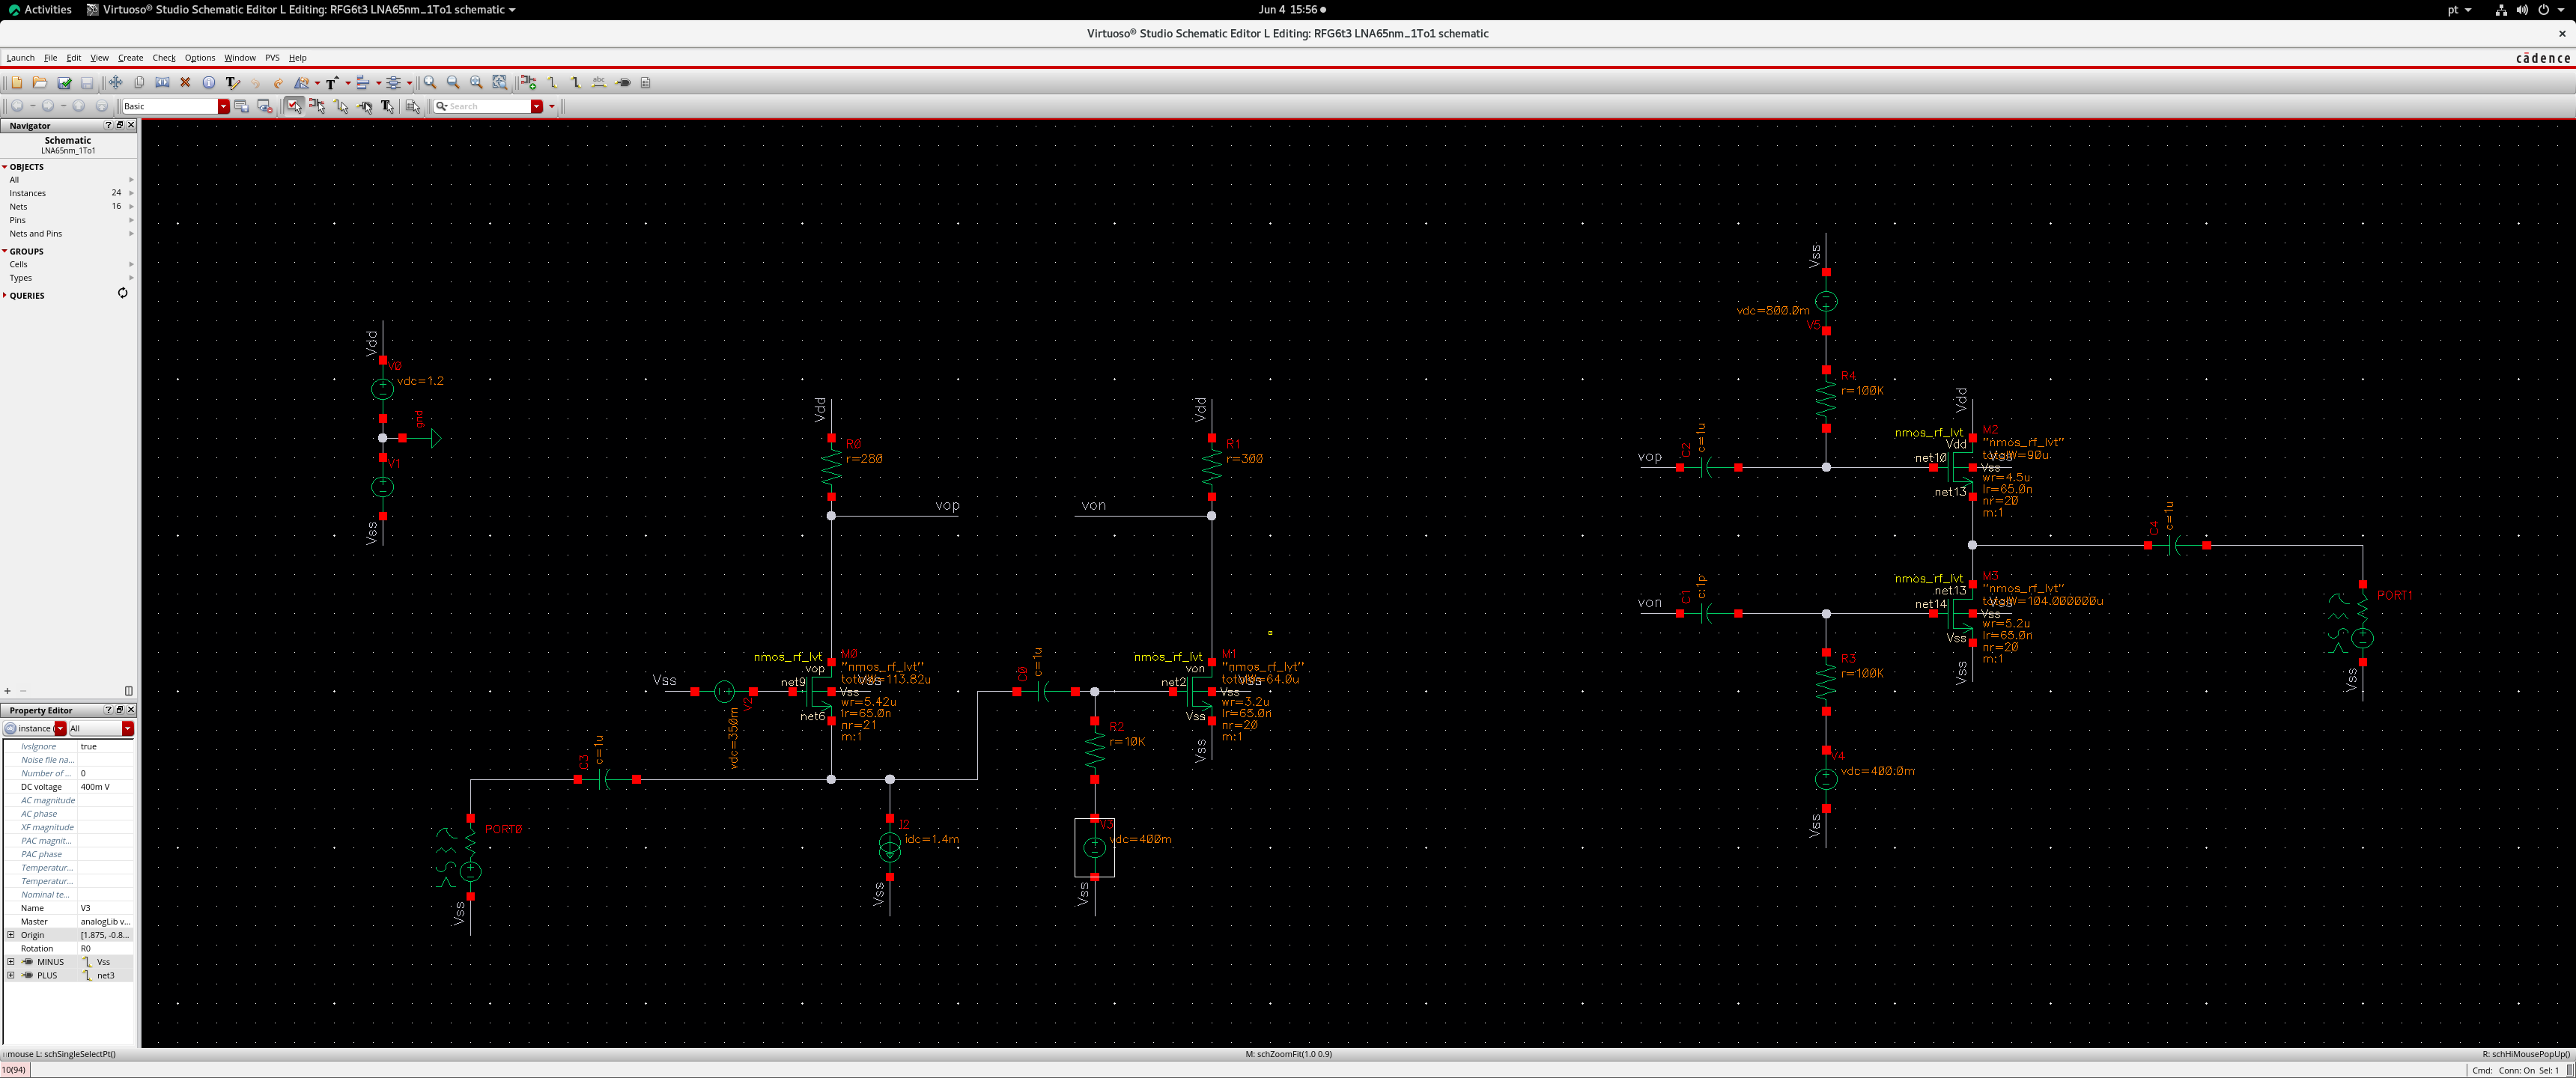
\includegraphics[width=1\textwidth]{Images/65nm1To1Circ.png}
    \caption{LNA Circuit for 65 nm Technology with 1:1 $g_m$ Ratio}
    \label{fig:65nm_1to1-circ}
\end{figure}

\begin{figure}[H]
    \centering
    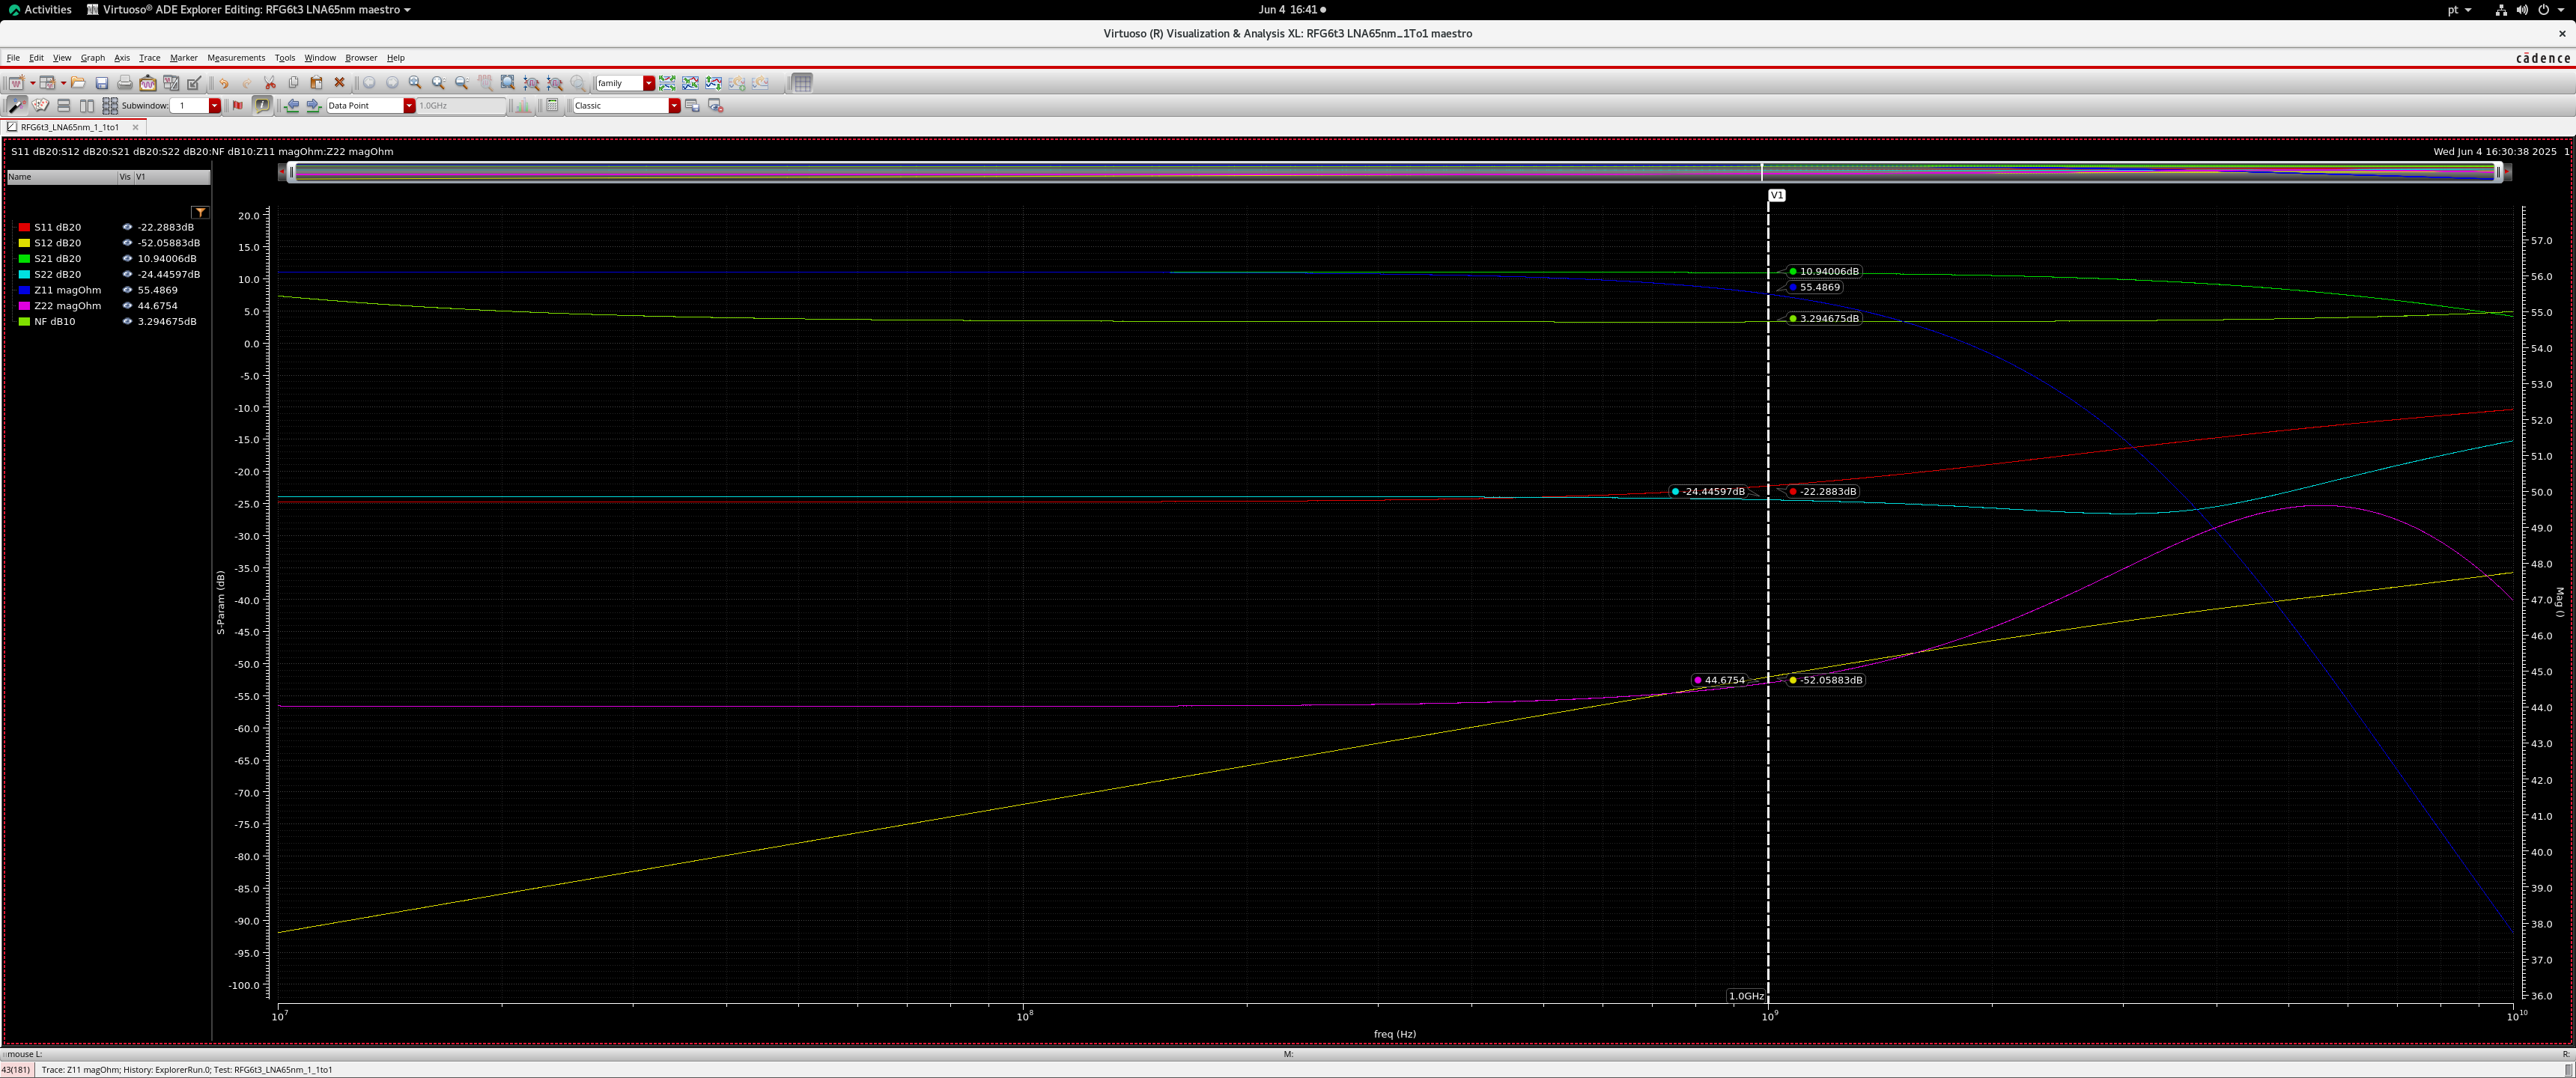
\includegraphics[width=1\textwidth]{Images/65nm1to1.png}
    \caption{LNA Simulation for 65 nm Technology with 1:1 $g_m$ Ratio}
    \label{fig:65nm_1to1}
\end{figure}

\begin{table}[H]
    \centering
    \caption{Simulation Results for 65 nm Technology with 1:1 $g_m$ Ratio}
    \begin{tabularx}{\textwidth}{>{\centering\arraybackslash}X >{\centering\arraybackslash}X }
        \toprule
        \textbf{Parameter} & \textbf{Value}\\
        \midrule
        Gain (S21) & 10.94\si{\decibel} \\
        \midrule
        Noise Figure (NF) & 3.29\si{\decibel} \\
        \midrule
        Input Impedance (Z11) & 44.68\si{ohm} \\
        \midrule
        Output Impedance (Z22) & 55.49\si{ohm} \\
        \bottomrule
    \end{tabularx}
    \label{tab:65nm_1to1_results}
\end{table}


\subsubsection{1:n $g_m$ ratio}

The circuit implemented in Cadence for the 65 nm technology with a 1:n $g_m$ ratio is shown in Figure \ref{fig:65nm_1ton-circ}. The simulation results are shown in Figure \ref{fig:65nm_1ton} summarized in Table \ref{tab:65nm_1ton_results}.

\begin{figure}[H]
    \centering
    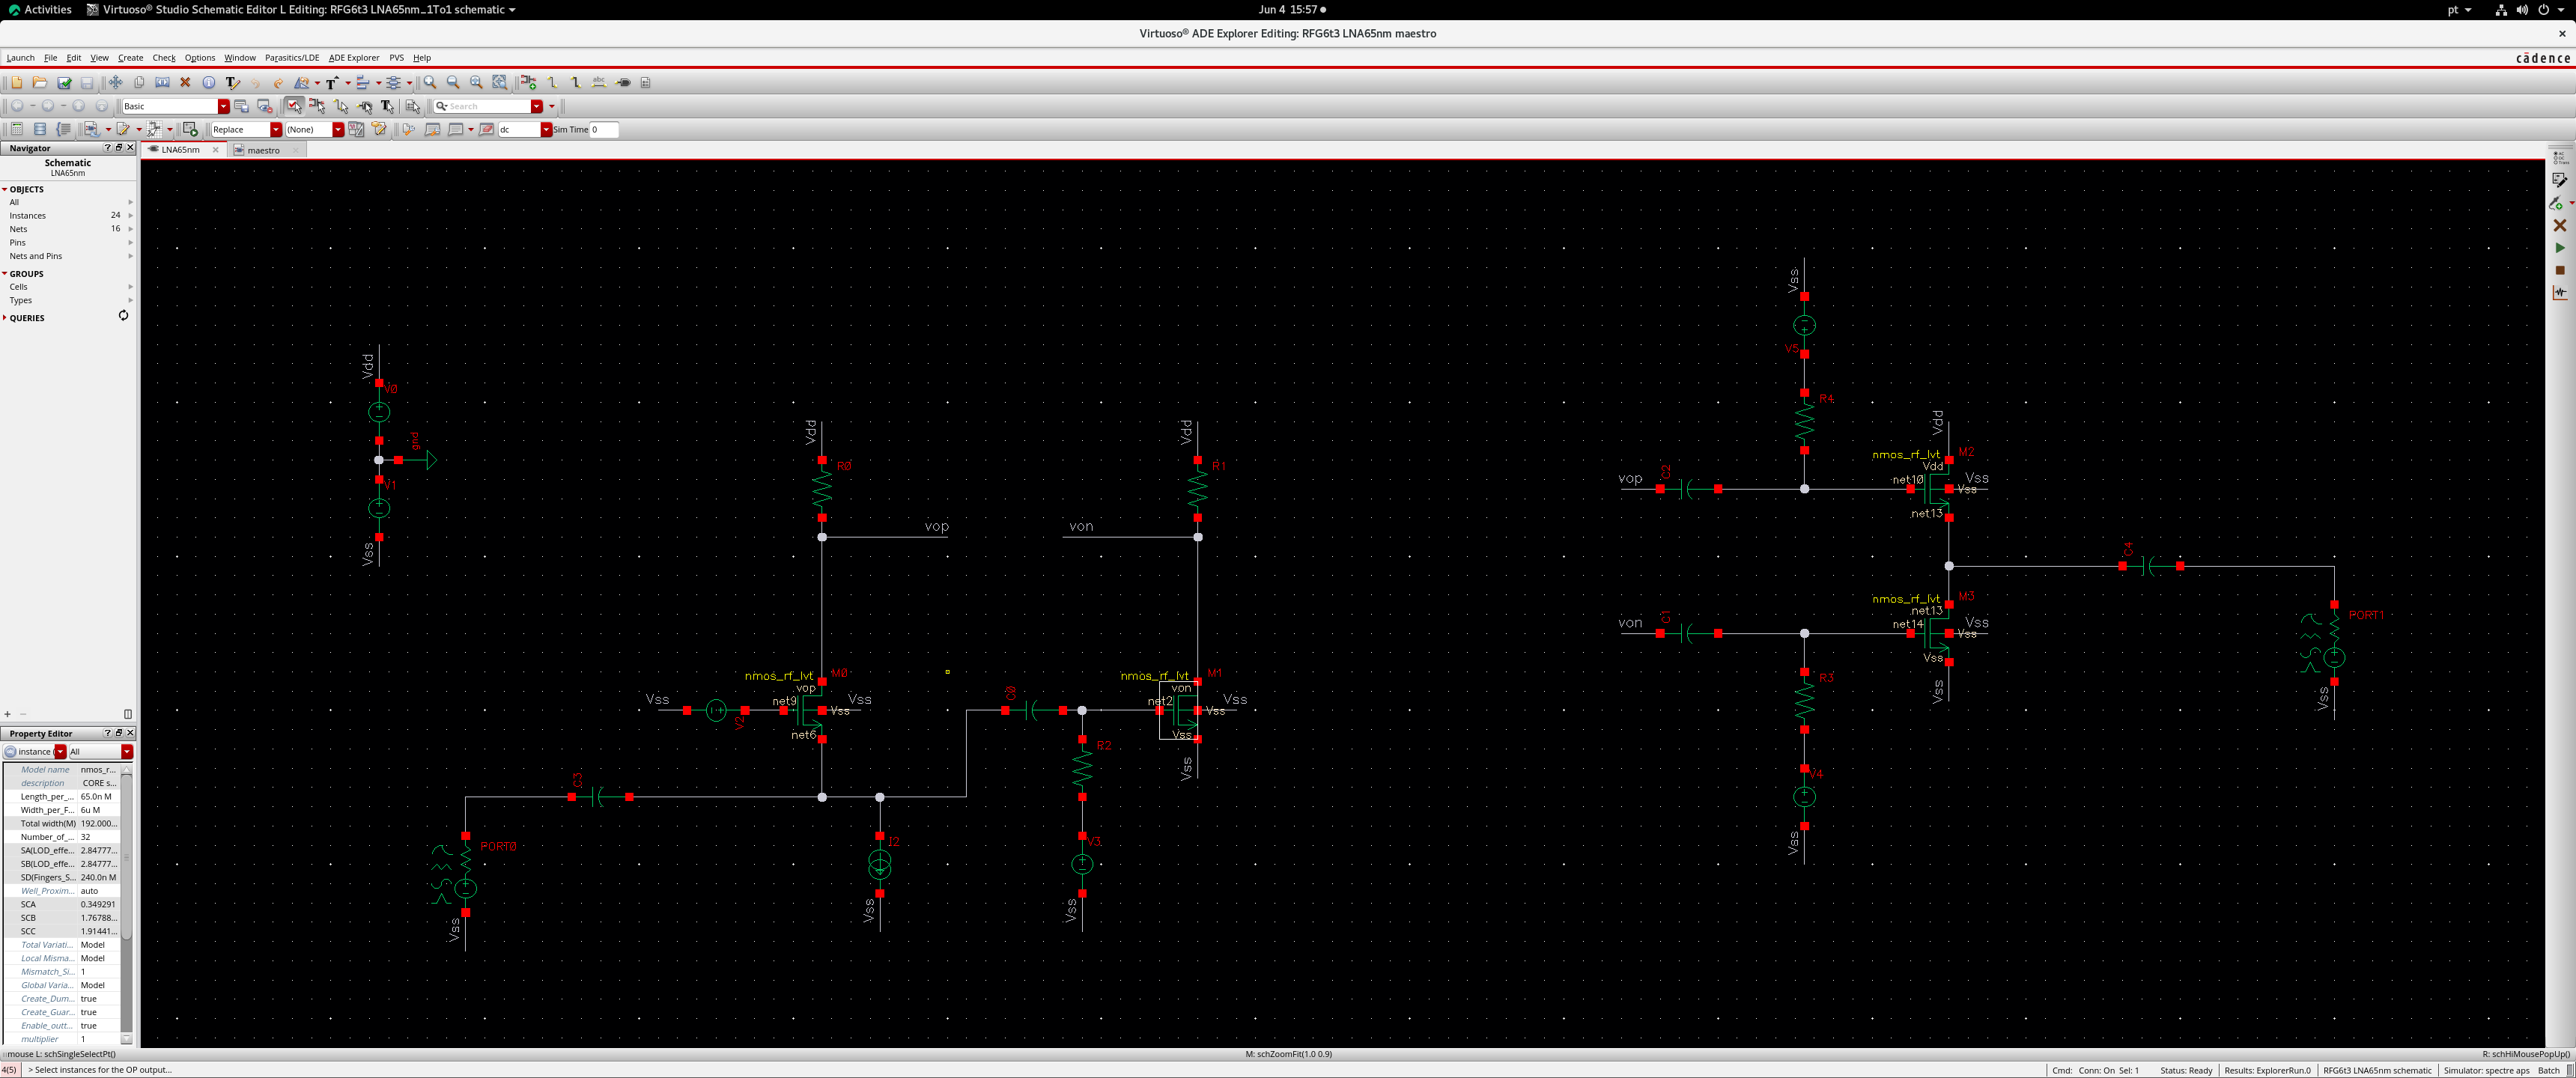
\includegraphics[width=1\textwidth]{Images/65nm1To35Circ.png}
    \caption{LNA Circuit for 65 nm Technology with 1:n $g_m$ Ratio}
    \label{fig:65nm_1ton-circ}
\end{figure}

\begin{figure}[H]
    \centering
    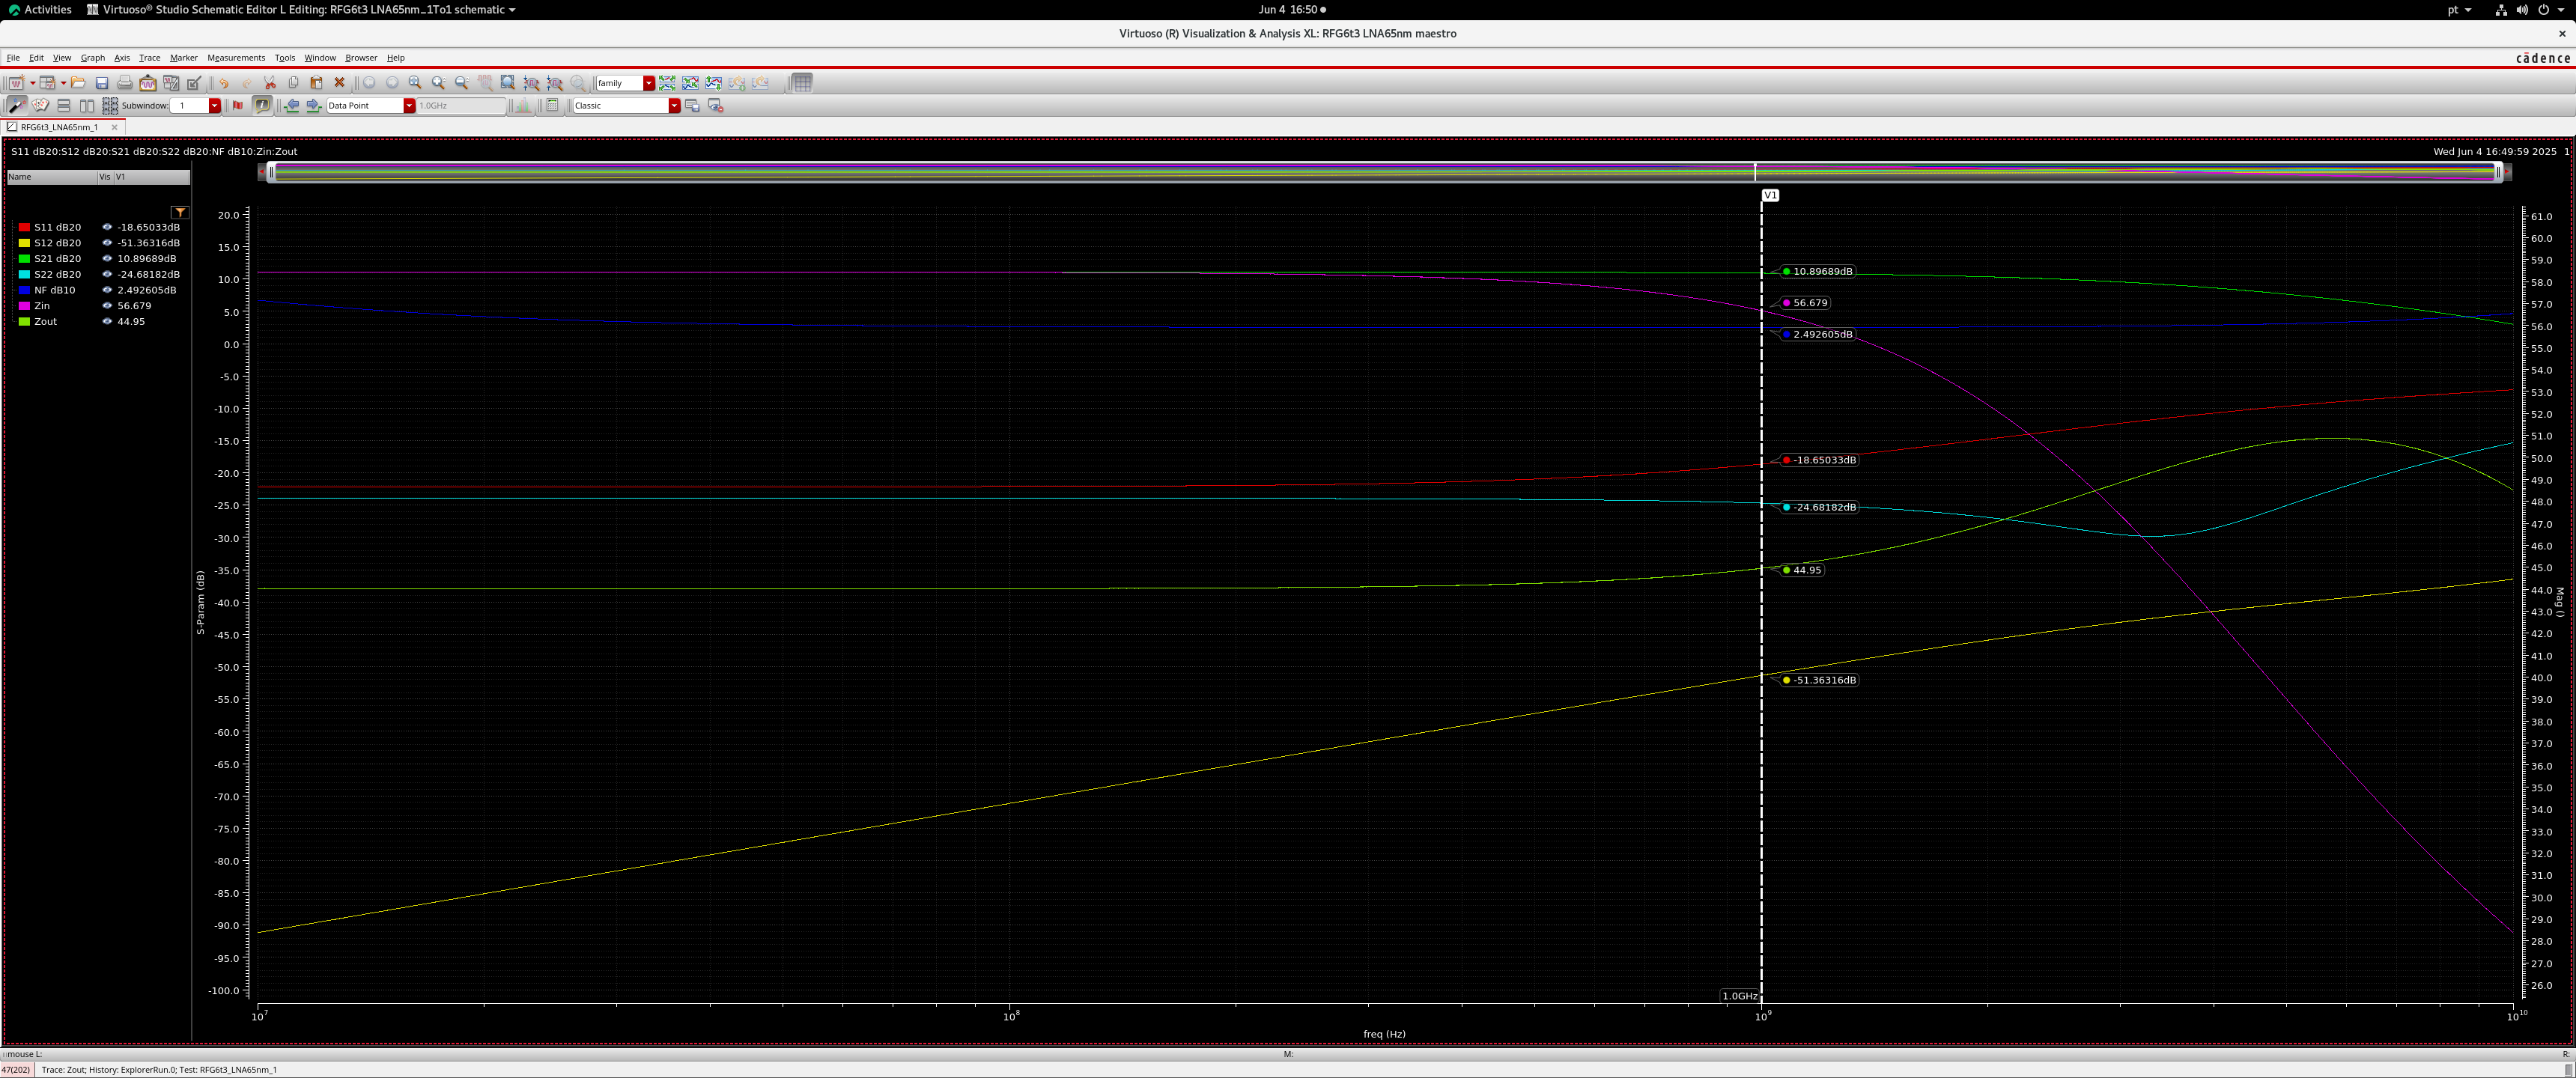
\includegraphics[width=1\textwidth]{Images/65nm1To35Final.png}
    \caption{LNA Simulation for 65 nm Technology with 1:n $g_m$ Ratio}
    \label{fig:65nm_1ton}
\end{figure}

\begin{table}[H]
    \centering
    \caption{Simulation Results for 65 nm Technology with 1:n $g_m$ Ratio}
    \begin{tabularx}{\textwidth}{>{\centering\arraybackslash}X >{\centering\arraybackslash}X }
        \toprule
        \textbf{Parameter} & \textbf{Value}\\
        \midrule
        Gain (S21) & \SI{10.86}{\decibel} \\
        \midrule
        Noise Figure (NF) & \SI{2.49}{\decibel} \\
        \midrule
        Input Impedance (Z11) & \SI{56.68}{\ohm} \\
        \midrule
        Output Impedance (Z22) & \SI{44.95}{\ohm} \\
        \bottomrule
    \end{tabularx}
    \label{tab:65nm_1ton_results}
\end{table}



\subsection{Simulation for 45 nm Technology}

\subsection{Results Analysis and Comparison}